\documentclass[12pt,a4paper]{article}

% ── Packages ──────────────────────────────────────────────────────────────────
\usepackage[T1]{fontenc}
\usepackage[utf8]{inputenc}



\usepackage{amsmath, amssymb, amsfonts, amsthm, mathtools}
\usepackage{graphicx}
\usepackage{geometry}
\usepackage{hyperref}
\usepackage{enumitem}
\usepackage{xcolor}
\usepackage{tcolorbox}
\usepackage{booktabs}
\usepackage{float}

\geometry{margin=2.5cm}

% ── Theorem environments ───────────────────────────────────────────────────────
\theoremstyle{definition}
\newtheorem{definition}{Définition}[section]
\newtheorem{exemple}{Exemple}[section]

\theoremstyle{plain}
\newtheorem{theoreme}{Théorème}[section]
\newtheorem{proposition}{Proposition}[section]
\newtheorem{lemme}{Lemme}[section]

\theoremstyle{remark}
\newtheorem{remarque}{Remarque}[section]
\newtheorem{observation}{Observation}[section]

% ── Shortcuts ─────────────────────────────────────────────────────────────────
\newcommand{\CC}{\mathbb{C}}
\newcommand{\RR}{\mathbb{R}}
\newcommand{\NN}{\mathbb{N}}
\newcommand{\DD}{\mathbb{D}}
\newcommand{\Sp}{\mathrm{Sp}}
\newcommand{\norm}[1]{\left\|#1\right\|}
\newcommand{\abs}[1]{\left|#1\right|}
\newcommand{\dbar}{\bar{\partial}}
\DeclareMathOperator{\rot}{rot}

% ── Document ──────────────────────────────────────────────────────────────────
\title{\textbf{Analyse complexe et applications à l'algèbre linéaire}\\[0.5em]
       \large Notes de cours}
\author{}
\date{}

\begin{document}
\maketitle
\tableofcontents
\newpage

% ══════════════════════════════════════════════════════════════════════════════
\section{Résolvante et spectre}
% ══════════════════════════════════════════════════════════════════════════════

\subsection{Définitions}

\begin{definition}[Spectre et résolvante]
Soit $A \in M_n(\CC)$. On appelle \emph{spectre} de $A$ l'ensemble
\[
  \Sp(A) = \{\, \mu \in \CC \mid A - \mu I \text{ n'est pas inversible}\,\}.
\]
Pour tout $\lambda \in \CC \setminus \Sp(A)$, la matrice $A - \lambda I$ est inversible.
On note
\[
  R_A(\lambda) = (A - \lambda I)^{-1}
\]
et on l'appelle la \emph{résolvante} de $A$ en $\lambda$.
\end{definition}

\begin{remarque}
On dispose d'une expression alternative. Posons
\[
  B_A(z) = (I - zA)^{-1}, \qquad z \in \CC \setminus \bigl\{\tfrac{1}{\mu} \mid \mu \in \Sp(A)\bigr\}.
\]
Un calcul direct donne
\[
  R_A(\lambda) = -\frac{1}{\lambda}\, B_A\!\left(\frac{1}{\lambda}\right).
\]
\end{remarque}

\subsection{Norme d'opérateur}

On munit $\CC^n$ de la norme euclidienne $\norm{\cdot}_2$. La \emph{norme d'opérateur}
(norme subordonnée) d'une matrice $A \in M_n(\CC)$ est
\[
  \norm{A} = \sup_{\substack{v \in \CC^n \\ v \neq 0}} \frac{\norm{Av}_2}{\norm{v}_2}.
\]
Elle satisfait en particulier
\[
  \norm{AB} \leq \norm{A}\,\norm{B}.
\]
De plus, si $\norm{A} < 1$ alors $I - A$ est inversible et
\[
  (I-A)^{-1} = \sum_{n=0}^{+\infty} A^n.
\]

\subsection{Développement en série entière de la résolvante}

\begin{proposition}
\label{prop:serie-resolvante}
La série suivante converge (localement uniformément pour la norme d'opérateur)
sur le disque $\DD\!\left(0,\,\frac{1}{\norm{A}}\right)$\,:
\[
  B_A(z) = \sum_{n=0}^{+\infty} z^n A^n.
\]
(Poly, Prop.\ 4.8)
\end{proposition}

\begin{figure}[H]
  \centering
  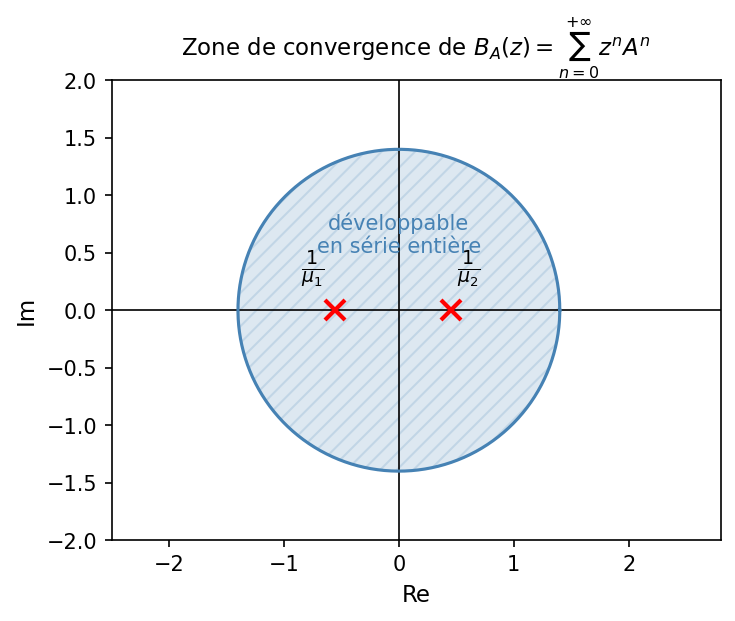
\includegraphics[width=0.52\textwidth]{figures/fig_resolvent_disk.png}
  \caption{Zone de convergence de $B_A(z)=\sum_{n=0}^{+\infty}z^n A^n$.
           Les croix marquent les singularités $1/\mu_i$ pour $\mu_i\in\Sp(A)$.}
  \label{fig:resolvent-disk}
\end{figure}

\begin{remarque}
Au voisinage de tout point de son domaine de définition, la fonction $B_A$ est
développable en série entière, i.e.
\[
  B_A(z) = \sum_{n=0}^{+\infty} (z - z_0)^n\, B_A(z_0)\,\bigl[A\,B_A(z_0)\bigr]^n.
\]
\textbf{But :} étudier ce type de fonction d'une variable complexe.
\end{remarque}

Un calcul algébrique montre que
\[
  B_A(z)
  = (I - zA)^{-1}
  = \bigl(I - z_0 A - (z-z_0)A\bigr)^{-1}
  = (C - D)^{-1}
  = \sum_{n=0}^{+\infty} C^{-1}(DC^{-1})^n,
\]
où l'on a posé $C = I - z_0 A$ et $D = (z-z_0)A$.

% ══════════════════════════════════════════════════════════════════════════════
\section{Fonctions holomorphes}
% ══════════════════════════════════════════════════════════════════════════════

\subsection{Définition}

\begin{definition}[Fonction holomorphe]
Soit $\Omega \subset \CC$ un ouvert et $f : \Omega \to \CC$.
On dit que $f$ est \emph{holomorphe} lorsque
\[
  \forall\, z_0 \in \Omega,\quad
  \exists\, \varepsilon > 0
  \text{ et une suite } (a_n)_{n \in \NN}
  \text{ tels que }
  \forall\, z \in \DD(z_0, \varepsilon),\quad
  f(z) = \sum_{n=0}^{+\infty} a_n (z - z_0)^n.
\]
\end{definition}

\subsection{Rappel : convergence des séries entières}

\begin{proposition}[Piqûre de rappel]
Si $(|a_n|^{1/n})_{n\in\NN}$ est bornée par $M > 0$, alors la série entière
\[
  z \mapsto \sum_{n \in \NN} a_n z^n
\]
converge localement uniformément sur $\DD(0, 1/M)$, et définit une fonction
$C^\infty$ (en tant que fonction des deux variables réelles).

En particulier, si $R < \frac{1}{M}$ et $z \in \DD(0,R)$, alors
\[
  \sum_{n \in \NN} |a_n z^n| \leq \sum_{n \in \NN} (RM)^n < +\infty.
\]
\end{proposition}

\subsection{Observation : l'opérateur \texorpdfstring{$\dbar$}{d-bar}}

\begin{observation}
En écrivant $z = x + iy$, on calcule les dérivées partielles des monômes :
\[
  \frac{\partial}{\partial x}(x+iy)^n = n(x+iy)^{n-1},
  \qquad
  \frac{\partial}{\partial y}(x+iy)^n = in(x+iy)^{n-1}.
\]
En particulier, pour tout $n \in \NN$,
\[
  \left(\frac{\partial}{\partial x} + i\frac{\partial}{\partial y}\right)(x+iy)^n = 0.
\]
On note $\dbar = \frac{\partial}{\partial \bar{z}} = \frac{1}{2}\!\left(\frac{\partial}{\partial x} + i\frac{\partial}{\partial y}\right)$
(aussi noté $\frac{\partial}{\partial \bar{z}}$).
\end{observation}

\begin{proposition}
\label{prop:dbar}
Si $f$ est holomorphe, alors $\dbar f = 0$.
\end{proposition}

\subsection{Exemples}

Les fonctions suivantes sont holomorphes :
\begin{itemize}[leftmargin=2em]
  \item la résolvante $\lambda \mapsto R_A(\lambda)$,
  \item les polynômes,
  \item l'exponentielle $z \mapsto \exp(z)$,
  \item la matrice-exponentielle $z \mapsto \exp(zA)$.
\end{itemize}

\begin{exemple}[Non-exemple]
La fonction $z \mapsto \bar{z}$ \emph{n'est pas} holomorphe car
\[
  \frac{\partial}{\partial x}(x - iy) = 1, \qquad
  \frac{\partial}{\partial \bar{z}}(x - iy) = 1 \neq 0.
\]
\end{exemple}

% ══════════════════════════════════════════════════════════════════════════════
\section{Intégrales de contour}
% ══════════════════════════════════════════════════════════════════════════════

\subsection{Formule de Stokes / Théorème d'Ampère}

\subsubsection{Version 1D}

Si $f \in C^1([a,b], \RR)$, alors
\[
  \int_a^b f'(x)\,dx = f(b) - f(a).
\]

\subsubsection{Version 2D}

Soit $\Omega \subset \RR^2$ un ouvert dont le bord est une courbe régulière simple $\gamma$.
On parcourt $\gamma$ à vitesse $1$ ; on note $T = \text{Longueur}(\gamma)$.

\begin{figure}[H]
  \centering
  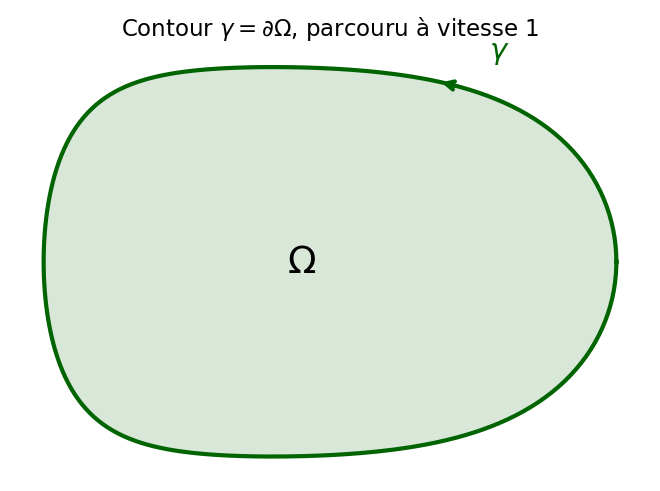
\includegraphics[width=0.38\textwidth]{figures/fig_contour_simple.png}
  \caption{Contour simple $\gamma = \partial\Omega$ orienté dans le sens direct.}
  \label{fig:contour-simple}
\end{figure}

\begin{theoreme}[Stokes / Green-Riemann]
\label{thm:stokes}
Soit $\vec{A} : \Omega \to \RR^2$ un champ de vecteurs $C^1$, avec
\[
  \vec{A}(x,y) = A_x(x,y)\,\vec{e}_x + A_y(x,y)\,\vec{e}_y.
\]
On définit le rotationnel scalaire
\[
  \rot(\vec{A}) = \frac{\partial A_y}{\partial x} - \frac{\partial A_x}{\partial y}.
\]
Alors
\[
  \iint_\Omega \rot(\vec{A})\,dx\,dy
  = \int_0^T \vec{A}(\gamma(s)) \cdot \vec{T}(\gamma(s))\,ds,
\]
où $\vec{T}(s) = \gamma'(s)$ est le vecteur tangent unitaire.
\end{theoreme}

\subsubsection{Preuve sur le carré}

Pour illustrer, on prend $\Omega = [0,1]^2$ (un carré) et $A$ affine :
\[
  A_x = c_x + a_{xx}\,x + a_{xy}\,y, \qquad A_y = c_y + a_{yx}\,x + a_{yy}\,y.
\]
Ainsi $\rot(\vec{A}) = a_{yx} - a_{xy}$, donc
\[
  \iint_\Omega \rot(\vec{A}) = a_{yx} - a_{xy}.
\]

\begin{figure}[H]
  \centering
  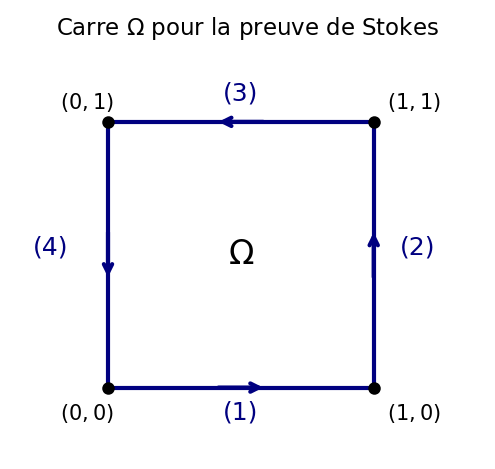
\includegraphics[width=0.38\textwidth]{figures/fig_square_stokes.png}
  \caption{Le carré $\Omega = [0,1]^2$ avec ses quatre côtés numérotés.}
  \label{fig:square-stokes}
\end{figure}

On paramétrise les quatre côtés :
\begin{align*}
  \text{Côté (1):} &\quad s \mapsto (s, 0),\quad s\in[0,1],
    & \int_0^1 A_x(s,0)\,ds &= c_x + \tfrac{a_{xx}}{2},\\
  \text{Côté (2):} &\quad s \mapsto (1, s),\quad s\in[0,1],
    & \int_0^1 A_y(1,s)\,ds &= c_y + a_{yx} + \tfrac{a_{yy}}{2},\\
  \text{Côté (3):} &\quad s \mapsto (1{-}s, 1),\quad s\in[0,1],
    & -\int_0^1 A_x(1{-}s,1)\,ds &= -(c_x + a_{xy} + \tfrac{a_{xx}}{2}),\\
  \text{Côté (4):} &\quad s \mapsto (0, 1{-}s),\quad s\in[0,1],
    & -\int_0^1 A_y(0,1{-}s)\,ds &= -(c_y + \tfrac{a_{yy}}{2}).
\end{align*}
En additionnant :
\[
  \oint_{\partial\Omega} \vec{A}\cdot d\vec{T}
  = a_{yx} - a_{xy}
  = \iint_\Omega \rot(\vec{A}).
\]
\textbf{Chemin vers une vraie preuve :}
\begin{enumerate}
  \item Vérifier d'abord pour des fonctions affines sur des triangles quelconques.
  \item Approcher $\gamma$ par une courbe polygonale, trianguler $\Omega$,
        et approcher $A$ par une fonction affine sur chaque triangle.
\end{enumerate}

\subsection{Intégrale complexe et formule de Green}

Soit $f : \Omega \to \CC$ de classe $C^1$ et $\gamma : [0,T] \to \CC$ une courbe régulière.
On définit l'intégrale complexe
\[
  \int_\gamma f = \int_0^T f(\gamma(s))\,\gamma'(s)\,ds.
\]

En posant $\vec{A}(x,y) = f(x,y)\,\vec{e}_x + if(x,y)\,\vec{e}_y$, on obtient :
\[
  \rot(\vec{A})
  = \frac{\partial(if)}{\partial x} - \frac{\partial f}{\partial y}
  = i\frac{\partial f}{\partial x} - \frac{\partial f}{\partial y}
  = i\!\left(\frac{\partial f}{\partial x} + i\frac{\partial f}{\partial y}\right)
  = i\cdot 2\dbar f.
\]

\begin{proposition}
\label{prop:green-complex}
Si $f : \Omega \to \CC$ est de classe $C^1$ et $\dbar f = 0$, alors pour toute
courbe $\gamma : [0,T] \to \CC$ fermée (i.e.\ $\gamma(0) = \gamma(T)$),
\[
  \int_0^T f(\gamma(s))\,\gamma'(s)\,ds = 0.
\]
En d'autres termes, $\displaystyle\oint_\gamma f = 0$.
\end{proposition}

\begin{remarque}
Il suffit d'avoir une courbe simple et $f$ définie partout à l'intérieur.
En général, pour des contours plus complexes :
\[
  \oint_{\gamma_1} f = 0
  \qquad\text{et}\qquad
  \oint_{\gamma_2} f = \oint_{\gamma_3} f.
\]
\end{remarque}

\begin{figure}[H]
  \centering
  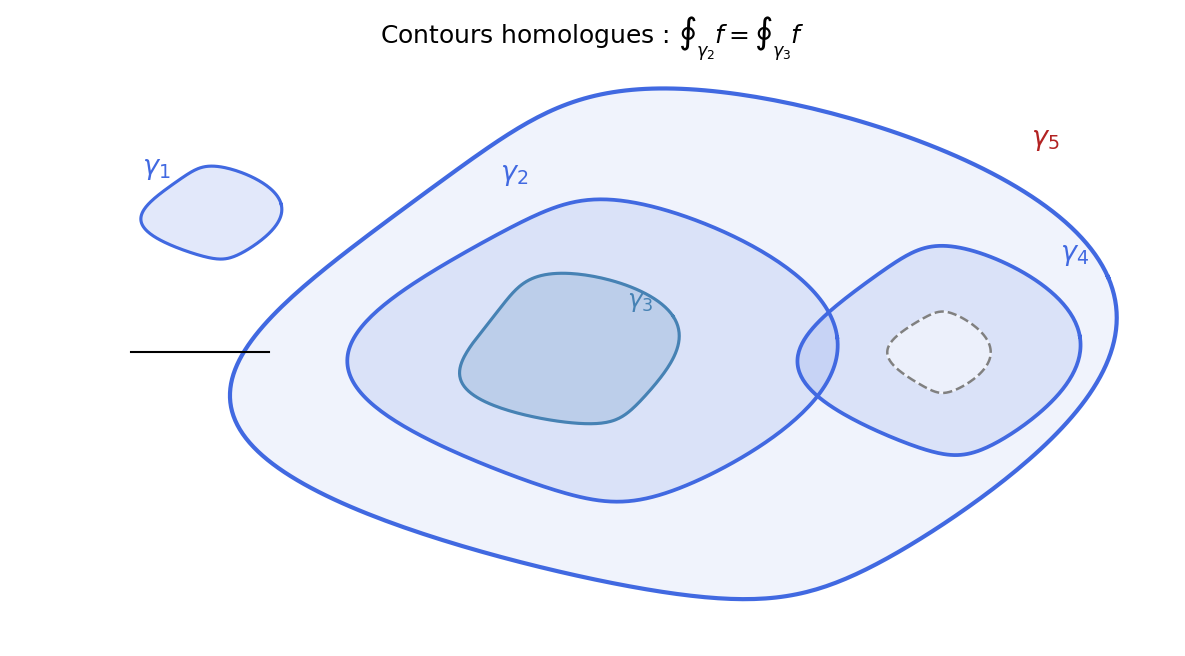
\includegraphics[width=0.70\textwidth]{figures/fig_nested_contours.png}
  \caption{Contours homologues : $\gamma_1$ (petit contour isolé),
           $\gamma_2, \gamma_3$ (contours emboîtés sur la gauche),
           $\gamma_4$ (contour avec trou),
           $\gamma_5$ (grand contour extérieur).
           On a $\oint_{\gamma_2} f = \oint_{\gamma_3} f$ et
           $\oint_{\gamma_5} f = \oint_{\gamma_2} f + \oint_{\gamma_4} f$.}
  \label{fig:nested-contours}
\end{figure}

Lorsque $\gamma_5 = \gamma_2 \cup \gamma_4$ (avec coupures), on a
\[
  \oint_{\gamma_5} f = \oint_{\gamma_2} f + \oint_{\gamma_4} f.
\]

% ══════════════════════════════════════════════════════════════════════════════
\section{Formule de Cauchy}
% ══════════════════════════════════════════════════════════════════════════════

\subsection{Énoncé}

\begin{theoreme}[Formule de Cauchy]
\label{thm:cauchy}
Soit $f \in C^1(\Omega, \CC)$ avec $\dbar f = 0$.
Soit $z_0 \in \Omega$. Alors, pour toute courbe $\gamma$ qui fait un tour
(dans le sens direct) autour de $z_0$,
\[
  \oint_\gamma \frac{f(z)}{z - z_0}\,dz = 2\pi i\, f(z_0).
\]
\end{theoreme}

\subsection{Preuve}

La valeur de l'intégrale ne dépend pas de $\gamma$, donc on prend $\gamma_\varepsilon$
le cercle de rayon $\varepsilon$ autour de $z_0$ :
\[
  \oint_{\gamma_\varepsilon} \frac{f(z)}{z - z_0}\,dz
  = \oint_{\gamma_\varepsilon} \frac{f(z_0)}{z - z_0}\,dz
    + O\!\left(\varepsilon \cdot \frac{1}{\varepsilon} \cdot \varepsilon\right)
  = O(\varepsilon).
\]

\begin{figure}[H]
  \centering
  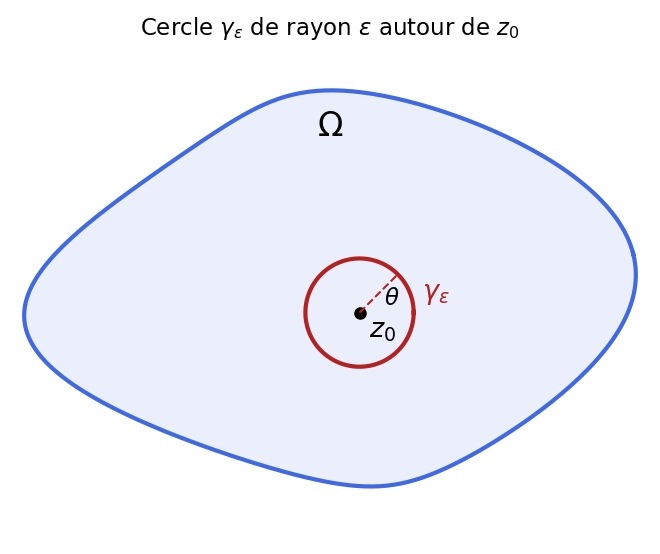
\includegraphics[width=0.44\textwidth]{figures/fig_cauchy_circle.png}
  \caption{Le cercle $\gamma_\varepsilon$ de rayon $\varepsilon$ centré en $z_0$,
           utilisé dans la preuve de la formule de Cauchy.}
  \label{fig:cauchy-circle}
\end{figure}

On calcule le terme principal. On paramétrise
$\gamma_\varepsilon : \theta \mapsto z_0 + \varepsilon e^{i\theta}$ pour $\theta \in [0, 2\pi]$.
Alors $\gamma_\varepsilon'(\theta) = i\varepsilon e^{i\theta}$ et
\[
  \oint_{\gamma_\varepsilon} \frac{1}{z - z_0}\,dz
  = \int_{\theta=0}^{2\pi}
      \frac{1}{\varepsilon e^{i\theta}} \cdot i\varepsilon e^{i\theta}\,d\theta
  = \int_0^{2\pi} i\,d\theta
  = 2\pi i.
\]

\subsection{Conséquence : caractérisation des fonctions holomorphes}

\begin{theoreme}
\label{thm:holo-dbar}
Soit $\Omega$ un ouvert de $\CC^2$, $f : \Omega \to \CC$ de classe $C^1$ telle
que $\dbar f = 0$. Alors $f$ est holomorphe.
\end{theoreme}

\begin{proof}
Soit $\gamma$ une courbe simple dans $\Omega$.
Pour tout $z_0 \in \omega$ (l'intérieur de $\gamma$), la formule de Cauchy donne
\[
  f(z_0) = \frac{1}{2\pi i} \oint_\gamma \frac{f(z)}{z - z_0}\,dz.
\]
Pour tout $z \in \gamma$, la fonction $z_0 \mapsto \frac{1}{z - z_0}$ est holomorphe
sur $\CC \setminus \{z\}$. Après intégration, $z_0 \mapsto \frac{1}{2\pi i}\oint_\gamma \frac{f(z)}{z-z_0}\,dz$
est holomorphe sur $\omega$.
\end{proof}

% ══════════════════════════════════════════════════════════════════════════════
\section{Application à l'algèbre linéaire}
% ══════════════════════════════════════════════════════════════════════════════

\subsection{Projecteur spectral}

\begin{proposition}[Projecteur sur un espace propre]
Soit $A \in M_n(\CC)$ diagonalisable, et soit $\gamma$ une courbe qui fait un tour
autour d'une valeur propre $\mu$, sans encercler les autres valeurs propres.
Alors
\[
  \frac{1}{2\pi i} \oint_\gamma R_A(z)\,dz = \Pi_\mu,
\]
où $\Pi_\mu$ est le \emph{projecteur} sur l'espace propre $E_\mu$, parallèlement
aux autres espaces propres.
\end{proposition}

\begin{figure}[H]
  \centering
  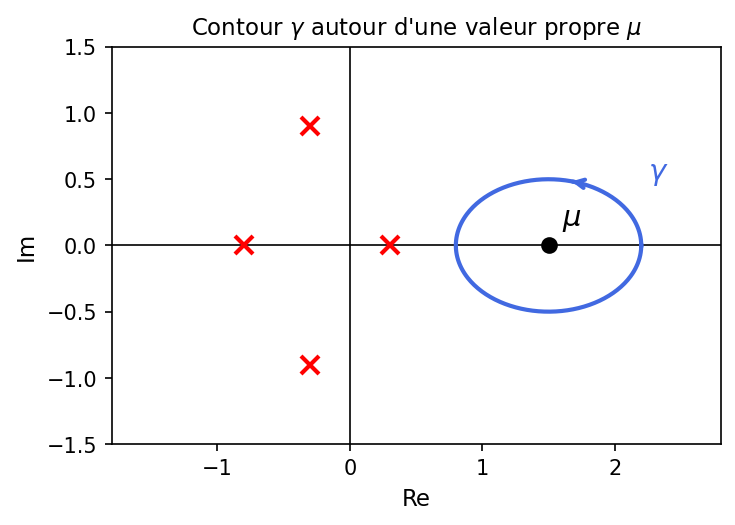
\includegraphics[width=0.48\textwidth]{figures/fig_eigenvalue_contour.png}
  \caption{Contour $\gamma$ entourant la valeur propre $\mu$ dans le plan complexe,
           sans encercler les autres valeurs propres (croix rouges).}
  \label{fig:eigenvalue-contour}
\end{figure}

\subsection{Preuve}

Puisque $A$ est diagonalisable, il existe $P$ inversible telle que
\[
  A = P^{-1}
      \begin{pmatrix} \mu & 0 \\ 0 & D' \end{pmatrix}
      P,
  \qquad \mu \notin \Sp(D').
\]
Alors
\[
  (A - \lambda I)^{-1}
  = P^{-1}
    \begin{pmatrix} (\mu - \lambda)^{-1} & 0 \\ 0 & (D'-\lambda I)^{-1} \end{pmatrix}
    P.
\]
On intègre sur $\gamma$ :
\[
  \frac{1}{2\pi i}\oint_\gamma (A-\lambda I)^{-1}\,d\lambda
  = P^{-1}
    \begin{pmatrix}
      \frac{1}{2\pi i}\oint_\gamma \frac{d\lambda}{\mu - \lambda} & 0 \\
      0 & 0
    \end{pmatrix}
    P
  = P^{-1}
    \begin{pmatrix} 1 & 0 \\ 0 & 0 \end{pmatrix}
    P
  = \Pi_\mu.
\]
Le bloc inférieur est nul car $(D' - \lambda I)^{-1}$ est holomorphe à l'intérieur de $\gamma$
(puisque $\mu \notin \Sp(D')$), et le bloc supérieur donne $2\pi i$ par calcul de résidu.

\end{document}
